% !TEX root = ../main.tex
\chapter{Reproducibility Details}\label{app:reproducibility}
\noindent\fbox{\parbox{0.97\linewidth}{\textbf{Code Availability.} The pipeline implementation is available at \url{https://github.com/mariusrueve/foldfusion}.}}

All experiments were executed on a Linux workstation with Python-based orchestration and locally installed DoGSite3, SIENA, LigandExtractor, and JAMDAscorer binaries. The runs used Ubuntu~24.04.3~LTS (Linux kernel~6.14.0-29-generic) on an AMD~Ryzen~7~7800X3D CPU with \SI{32}{\giga\byte} RAM, paired with an NVIDIA~GeForce~RTX~4070 discrete GPU (GNOME~46 on X11). Detailed operational instructions, including environment preparation, exact commands, and configuration snapshots, are provided in the accompanying documentation.

\paragraph{FoldFusion codebase.}
\begin{itemize}
    \item Project version: \texttt{foldfusion==0.1.0} (editable install)
    \item Python interpreter: CPython~3.12.3 within a virtual environment created via \texttt{python3 -m venv}
    \item pip version: \texttt{pip~24.0}
\end{itemize}

\paragraph{External executables.}
\begin{itemize}
    \item DoGSite3~1.1.0 \hfill (\texttt{/home/marius/Data/zbh/dogsite3\_1.1.0/dogsite3})
    \item SIENA~1.3.0 \hfill \makecell[l]{(\texttt{/home/marius/Data/zbh/siena\_1.3.0/siena}\\and \texttt{generate\_siena\_database})}
    \item LigandExtractor~2025-04 \hfill \makecell[l]{(\texttt{/home/marius/Data/zbh/}\\\texttt{LigandExtractor\_2025-04/ligand\_extractor})}
    \item JamdaScorer~1.0.0 \hfill (\texttt{/home/marius/Data/zbh/JamdaScorer\_1.0.0/JamdaScorer})
\end{itemize}

\paragraph{Python package stack (pip freeze).}
The following dependency snapshot was captured inside the project virtual environment immediately after the thesis experiments:

\begin{verbatim}
certifi==2025.8.3
charset-normalizer==3.4.3
contourpy==1.3.3
coverage==7.10.6
cycler==0.12.1
-e git+https://github.com/mariusrueve/foldfusion.git@
    9b5368810c268f79f19d92ba930f9485adbea2dc#egg=foldfusion
fonttools==4.60.0
idna==3.10
iniconfig==2.1.0
Jinja2==3.1.6
kiwisolver==1.4.9
MarkupSafe==3.0.2
matplotlib==3.10.6
mypy==1.18.1
mypy_extensions==1.1.0
narwhals==2.5.0
numpy==2.3.3
numpy-typing-compat==20250818.2.3
optype==0.13.4
packaging==25.0
pandas==2.3.2
pandas-stubs==2.3.2.250827
pathspec==0.12.1
pillow==11.3.0
plotly==6.3.0
pluggy==1.6.0
Pygments==2.19.2
pyparsing==3.2.4
pytest==8.4.2
pytest-cov==7.0.0
python-dateutil==2.9.0.post0
pytz==2025.2
requests==2.32.5
ruff==0.13.0
scipy==1.16.2
scipy-stubs==1.16.2.0
seaborn==0.13.2
six==1.17.0
tqdm==4.67.1
types-pytz==2025.2.0.20250809
types-requests==2.32.4.20250913
typing_extensions==4.15.0
tzdata==2025.2
urllib3==2.5.0
\end{verbatim}

The editable installation line documents the exact repository commit used for the experiments; package versions inherit the numbering emitted by \texttt{pip freeze}. When reproducing the pipeline, installing the dependencies above inside CPython~3.12.3 together with the listed external binaries suffices to recover the environment that produced the reported figures and tables.

Figure~\ref{fig:stage-runtime} summarizes per-stage runtimes for a stratified sample of \num{303} targets drawn from the production run (every eighth UniProt in lexicographic order). The distributions confirm that DoGSite3, SIENA, and JAMDAscorer remain within seconds per target under the hardware setup described above.

\begin{figure}[ht]
    \centering
    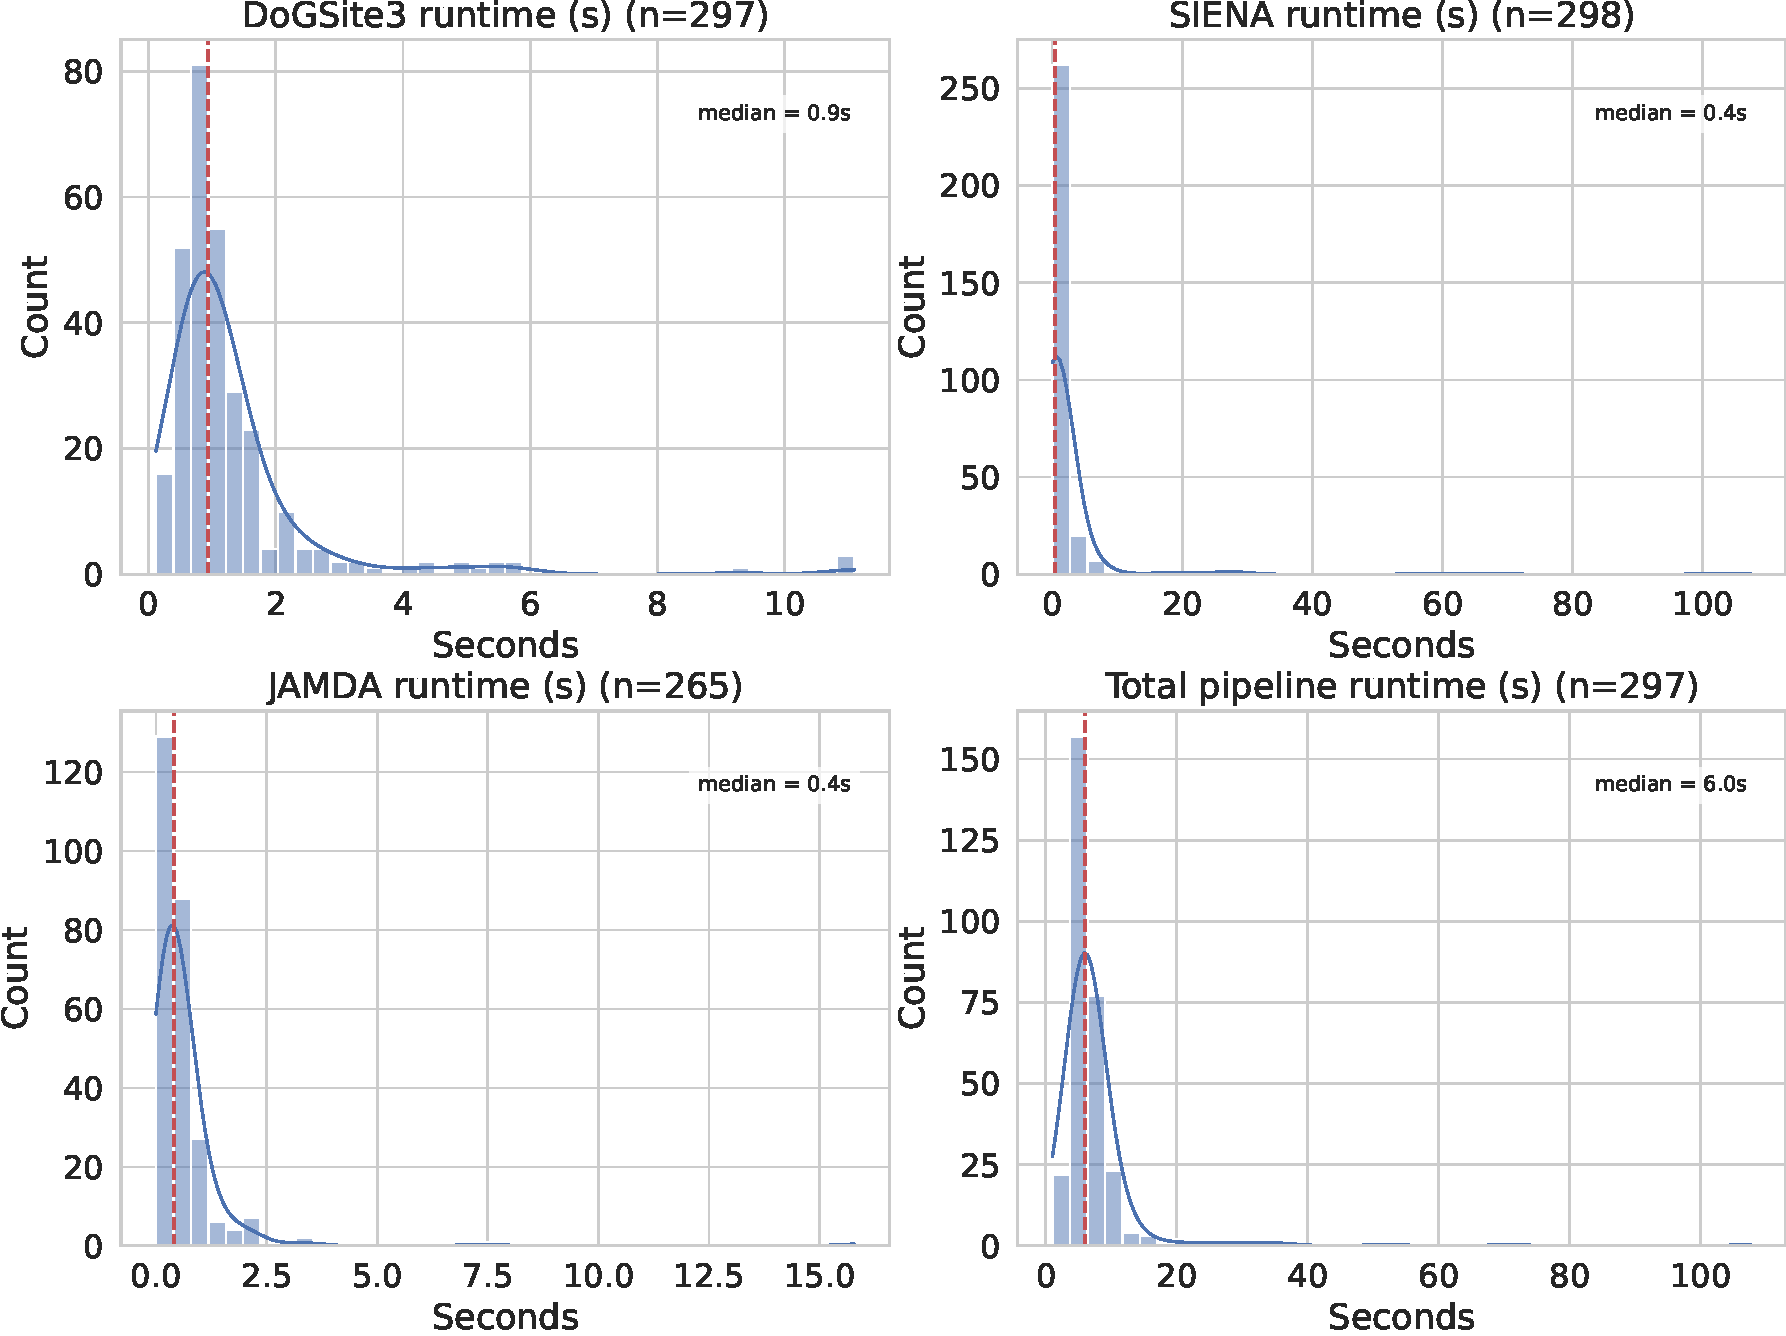
\includegraphics[width=0.9\linewidth]{figures/03_results/fig_stage_runtime_histograms.pdf}
    \caption[Stage runtime distributions]{Per-stage wall-time distributions across the \num{303}-target monitoring sample captured via stage-specific instrumentation. Vertical dashed lines mark medians, and sample sizes differ because DoGSite3 logs once per target, SIENA only when a donor aligns, and JAMDAscorer only when a placement is optimized.}
    \label{fig:stage-runtime}
\end{figure}

Table~\ref{tab:appendix-ion-breakdown} reports the ligand-class breakdown for the \num{6658} post-JAMDAscorer placements where \gls{tcs} metrics are defined. Monoatomic ions are counted separately because they are excluded from clash scoring, yielding \num{6488} organic placements (\SI{97.4}{\percent}) and \num{170} monoatomic ions (\SI{2.6}{\percent}) consistent with the Results chapter.

\begin{table}[ht]
\centering
\resizebox{\linewidth}{!}{%
\begin{tabular}{lrll}
\toprule
Category & Placements & Fraction & Notes \\
\midrule
Organic / polyatomic ligands & 6488 & \SI{97.4}{\percent} & Valid \gls{tcs} and \gls{lev} metrics available when donors provide references \\
Monoatomic ions & 170 & \SI{2.6}{\percent} & \gls{tcs} excluded from the main statistics; reported separately in plots \\
\bottomrule
\end{tabular}
}
\caption[Ligand class distribution]{Ligand-class distribution for the post-JAMDAscorer placements with defined \gls{tcs} metrics. Totals exclude cases where ligand extraction failed (none in the final run).}
\label{tab:appendix-ion-breakdown}
\end{table}


Licensing summary: DoGSite3 and SIENA are distributed for non-commercial academic research by the ZBH/University of Hamburg. JAMDAscorer is licensed for research use only. AlphaFold DB structures are provided under CC-BY~4.0, and mirrored PDB entries fall under the wwPDB data-use policy. Derived models should therefore be redistributed only with attribution to all upstream sources.
